% Chapter apnams

\chapter{APNA Management Service} % Main chapter title

\label{apnams} % For referencing the chapter elsewhere, use \ref{apnams}

\section{What is APNA Management Service}
APNA Management Service is a collection of four different types of services

\begin{itemize}
    \item Ephemeral ID Management Service
    \item Domain Name Service (DNS)
    \item Key Management Service (KMS)
    \item Identity Management Service (IMS)
\end{itemize}

\section{Ephemeral IDs Management} \label{sec:apna_ms}
Ephemeral IDs (EphIDs) are very important component needed for establishing anonymous and accountable communication between host. Thus a major responsibility of the management service is to issue this EphID very efficiently as it would be required by every host trying to establish a new communication. This should also meet the security guarantees that is required from EphIDs. In order to efficiently compute EphID instead of keeping huge mapping inside the table symmetric cryptography is used to implement it in a stateless fashion.

\subsection{Ephemeral ID (EphID) Structure}
We engineered the length of EphID to optimize processing for the AES block cipher as its the only cipher with widespread hardware support, which enables high performance. In order to generate EphIDs we use a CCA-secure encryption scheme. To this end, we use a generic composition called Encrypt-then-MAC that combines a symmetric encryption with a message authentication code (MAC).
Ephemeral IDs are composed of three things:
\begin{itemize}
    \item Initialization vector (IV)
    \item Encrypted Host Identifier (EHID)
    \item Message Authentication Code (MAC)
\end{itemize}

\begin{figure}[th]
\centering
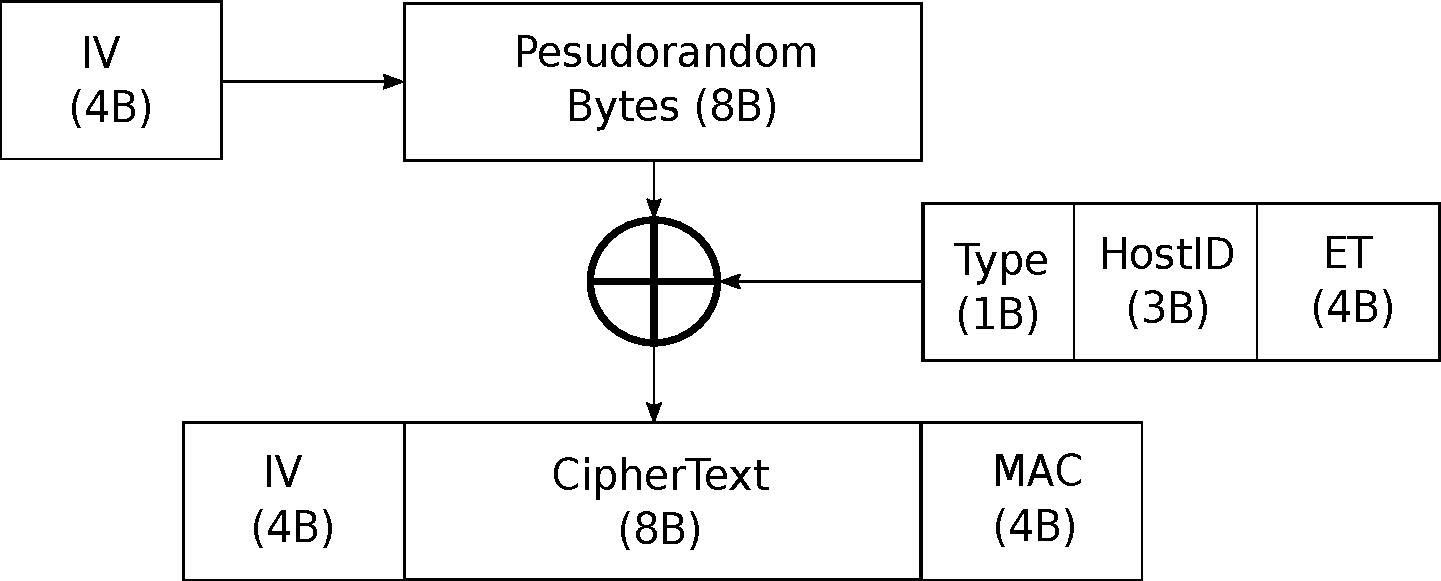
\includegraphics[scale=0.5]{Figures/ephid_construction.pdf}
\decoRule
\caption[EphID Construction]{EphID Construction, where ET is Expiration Time}
\label{fig:ephid_con}
\end{figure}

\subsubsection{Initialization Vector (IV)}
Secure operations of this mode in AES requires a unique IV for every encryption operation (i.e. for every EphID)

\subsubsection{Host Identifiers (HID)}
\begin{center}
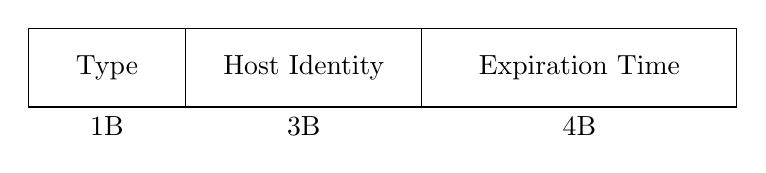
\begin{tikzpicture}
    \draw (0,0) rectangle (2,1) node[pos=.5] {Type}; %node[anchor=north, pos=.5]{0};
    \draw (2,0) rectangle (5,1) node[pos=.5] {Host Identity};
    \draw (5,0) rectangle (9,1) node[pos=.5] {Expiration Time};
    \draw (1 cm,0pt) -- (1 cm,0pt) node[anchor=north] {1B};
    \draw (3.5 cm,0pt) -- (3.5 cm,0pt) node[anchor=north] {3B};
    \draw (7 cm,0pt) -- (7 cm,0pt) node[anchor=north] {4B};
\end{tikzpicture}
\end{center}
Host Identifiers has three main components:
\begin{itemize}
    \item \textbf{Type:} There are two types Control EphID and Session EphID. Control EphID is mainly used to communicate with AS related services. On the other hand Session EphID is used for negotiating a session between client and server. It is also used during the whole communication process.
    \item \textbf{Host Identity:} Host is the 3 byte unique representation for all the host within the AS. It's sufficient enough to uniquely represent all host even in the large ASes.
    \item \textbf{Expiration Time:} This represents the validity of an EphID which is expressed in Unix seconds. Control EphID usually have a longer expiration time than Session EphID. For example in our implementation Control EphID has an expiration time of 1hour and Session EphID has an expiration time of 5mins.
\end{itemize}

\subsubsection{Message Authentication Code (MAC)}
IV and EHID are signed with the HMAC so that it could verify MAC before decryption of EphID to find HID to forward the packet.

\subsection{EphID Issuance} \label{sec:why_encrypt}
To obtain an EphID, the host generate public/private key pair ($K^{+}_{EphID}$, $K^{-}_{EphID}$) and send an EphID creation request to MS as shown in Figure \ref{fig:ephid_gen}. Specifically, the host first generates the key pairs for the EphID and include $K^{+}_{EphID}$ (\texttt{0xcafe}) along with type (\texttt{CtrlEphID}) and address of the domain name (\texttt{www.abc.com}) in the request message. All the communication with APNA Management Service is encrypted with using the shared key with the AS ($k_{HA}$). The public key in the message is encrypted to hide it from other entities in the AS that are not part of the AS infrastructure.

If an adversary trying to compromise sender-X unlinkability sees the content of EphID request packets, he/she can idenitfy a common sender at the level of $EphID_{Ctrl}$. Specifically the adversary first learns the ($EphID_{Ctrl}$, $K^{+}_{EphID}$) pair from the EphID request packets; then, the addversary sees the $K^{+}_{EphID}$ from the connection establishment packets, allowing the adversary to identify the common sender of multiple connections. Note that the actual host identity is still not compromised since only the host's AS can extract the host identity from $EphID_{Ctrl}$. In APNA, encrypting the EphID request message prevents such attacks.

Upon receiving the request, the EphID Mgmt Service validates the authenticity of the request; decrypts the source EphID ($EphID_{Ctrl}$) and performs the following check
\begin{itemize}
    \item $EphID_{Ctrl}$ has not expired
    \item the client's identifier ($HID$) is valid i.e, has not been revoked
    \item the request message is valid and can be decrypted successfully.
\end{itemize}
If anyone of them fails client gets a reply back with specific \textit{ErrorCode}. If its succesful then EphID Mgmt. Service generates an EphID and a certificate ($C_{EphID}$) corresponding to it and send it back as a response. The certificate is encrypted for the same reason as encrypting the EphID request packets.

\begin{figure}[th!!]
\centering
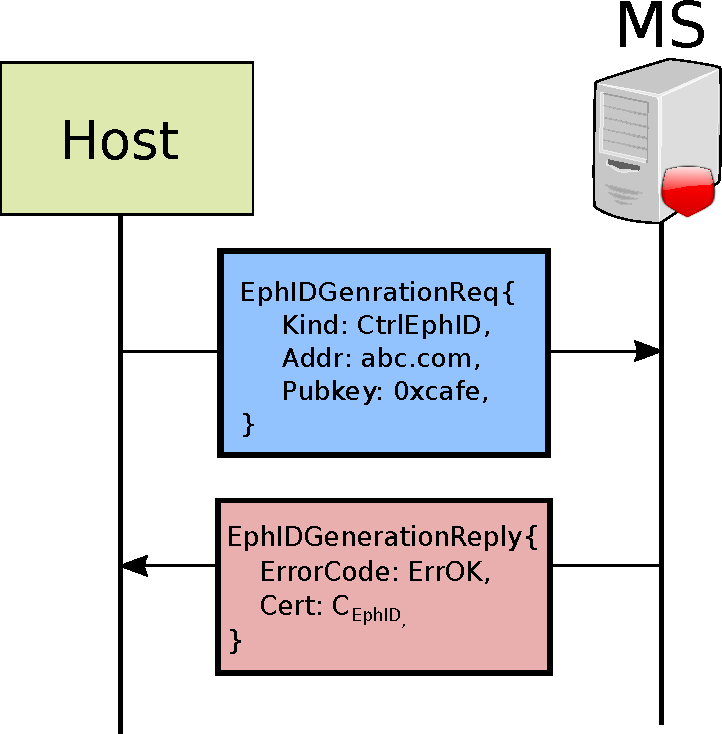
\includegraphics[scale=0.6]{Figures/ephid_gen.pdf}
\decoRule
\caption[EphID Generation Request]{Control EphID generation request by abc.com}
\label{fig:ephid_gen}
\end{figure}

\begin{figure}
    \centering
        \begin{bytefield}{32}
            \bitbox{32}{Ephemeral ID := $I_i$ (16 bytes)}\\
            \wordbox{1}{Pubkey (32 bytes)}\\
            \wordbox{1}{Expiration Time (4 bytes)}\\
            \bitbox{32}{Signature (32 bytes)}
        \end{bytefield}
        \decoRule
        \caption{Certificate byte level representation \tiny{\textsc{not to scale}}.}
        \label{fig:ephid_cert}
\end{figure}

\subsection{Certificate Structure}
In order to get more exact details about internals of the certificate associated with an EphID look at Figure \ref{fig:ephid_cert}. Signature is calculated using Elliptic Curve Cryptography (Ed25519) and thus the host can verify the authenticity of the issued certificate using the AS's public key which issued the certificate.

\section{Domain Name Service (DNS)} \label{sec:apna_dns}
\subsection{Why can't we use current DNS system?}
Since in APNA we have replaced IP addresses with Ephemeral Addresses which makes the current DNS system completely obsolete. Currently, DNS only understands how to resolve URL to IP addresses but in order to communicate with other APNA host we would need Ephemeral Address. In order to solve this problem current DNS could be modified be instead of returning A/AAAA records, it could return the certificate associated with the Ephemeral ID. This certificate contains all the details needed to establish the communication between communicating parties.

\subsection{Problems with publishing EphID to DNS}
Publishing EphIDs to the DNS raises a problem: a shutoff request against a published EphID would terminate any ongoing communication sessions that use this EphID. A naive solution is to update with a new EphID whenever published EphID becomes invalid. However an attacker can DDoS the DNS infrastructure by continuously sending shutoff request against a domain.

Our solution is to use Control EphIDs that are only used for to receive packets and are never used as the source EphIDs. Since they are never used as the source identifier, they cannot become the target of shutoff requests. To avoid using receive-only EphIDs as the source identifier, the communication establishment to a server needs to be changed (i.e., server does not respond to the client using the receive-only EphID).

\subsection{Details}
It's a simple prototype implementation for DNS which works on basic register and request based protocol. For instance a server could register its certificate associated with receive only EphID with DNS when it starts. Whenever a client would need to fetch the server identity it could request from DNS Service. Internally its implemented using Golang map data structure whose complexity for insertion and lookup is $\mathcal{O}(1)$ which makes it a perfect candidate for the prototype. This makes DNS operation very fast and efficient.

\subsection{DNS Operations}
\subsubsection{DNS Registration}
Figure \ref{fig:dns_register} represents a scenario in which a server registers \texttt{abc.com} receive only EphID's certificate ($C_{EphID}$) with the DNS service and if its successful it sends \texttt{ErrOk} back to the server.

\subsubsection{DNS Resolution}
Figure \ref{fig:dns_request} represents a scenario in which a client request for \texttt{abc.com} receive only EphID's certificate ($C_{EphID}$) with the DNS service and if the \texttt{abc.com} is registered with the DNS service it will reply with its $C_{EphID}$

\begin{figure}[th!]
\centering
\begin{subfigure}{.5\textwidth}
  \centering
  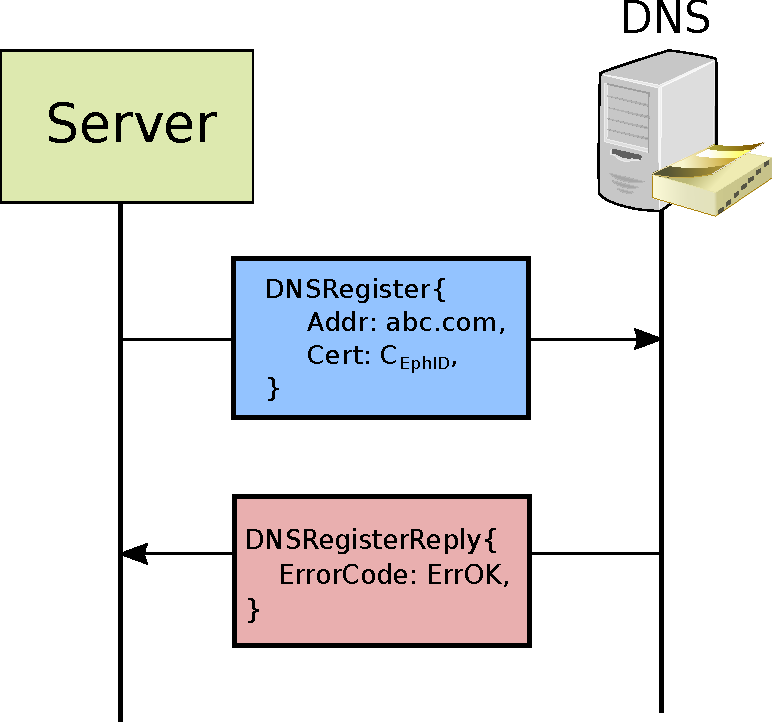
\includegraphics[width=0.95\linewidth]{Figures/dns_register.pdf}
  \caption[DNS Register Domain]{abc.com registers $C_{EphID}$ with DNS}
  \label{fig:dns_register}
\end{subfigure}%
\begin{subfigure}{.5\textwidth}
  \centering
  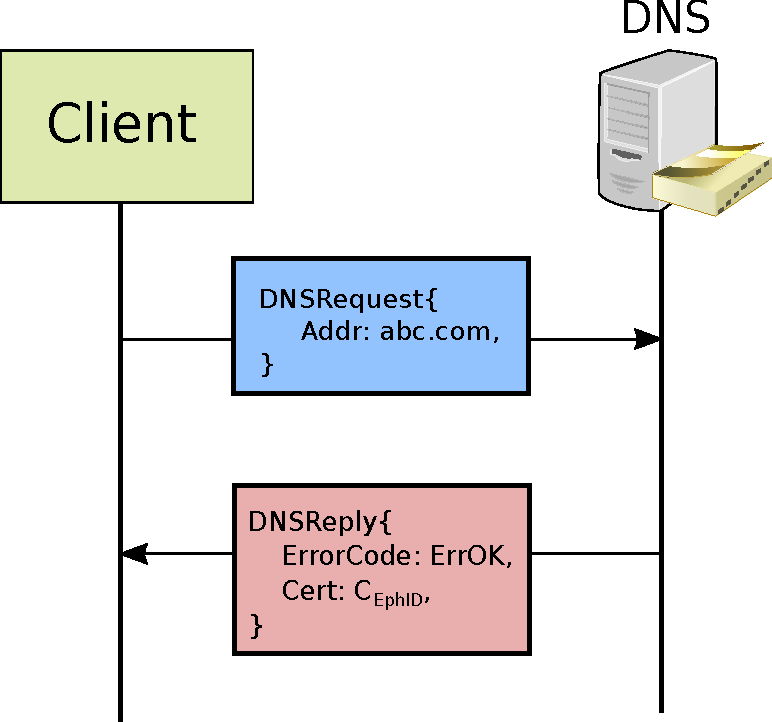
\includegraphics[width=0.95\linewidth]{Figures/dns_request.pdf}
  \caption[DNS Request for a Domain]{Client query abc.com's $C_{EphID}$ from DNS}
  \label{fig:dns_request}
\end{subfigure}
\caption{DNS Register and Request Methods}
\label{fig:dns}
\end{figure}

\section{Message Authentication Key Management} \label{sec:kms}
In APNA every packet contains MAC signed by the symmetric key of the host which is sending the packet. The symmetric key which is used to sign the packet is registered with the Management Service. So the forwarding service could ask the management service for this key and verify the authenticity of the packet before forwarding the packet to the rest of network.

\begin{figure}[th!]
\centering
\begin{subfigure}{.5\textwidth}
  \centering
  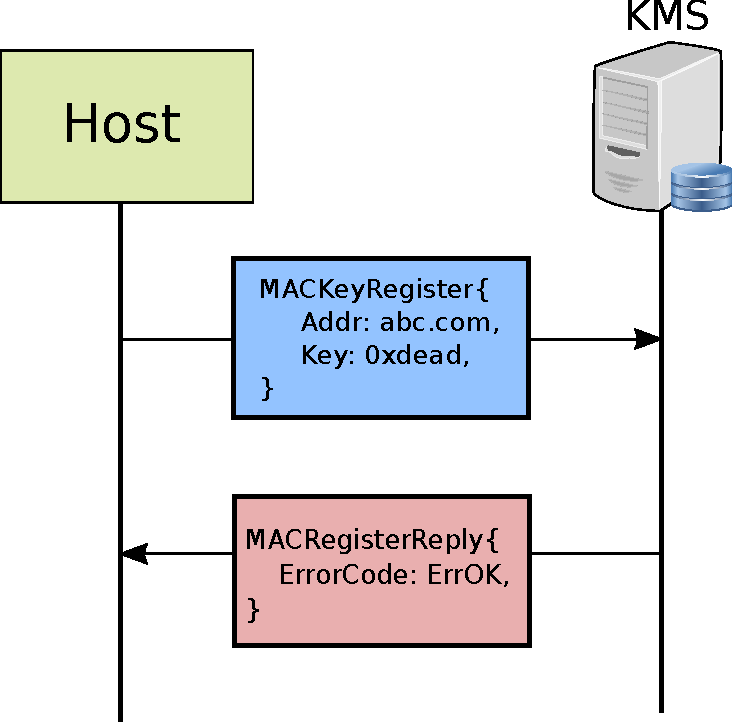
\includegraphics[width=0.95\linewidth]{Figures/kms.pdf}
  \caption[MAC Key Register]{Register Key}
  \label{fig:kms_register}
\end{subfigure}%
\begin{subfigure}{.5\textwidth}
  \centering
  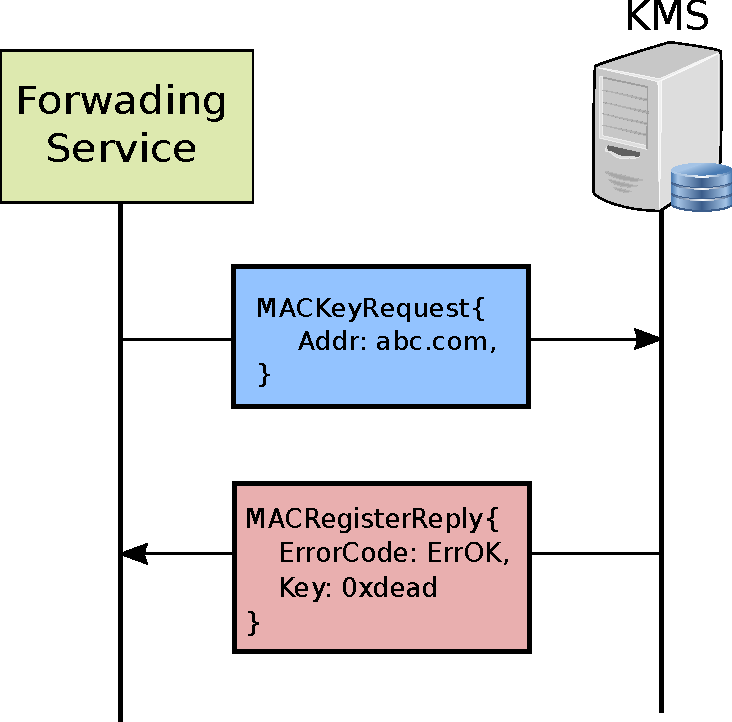
\includegraphics[width=0.95\linewidth]{Figures/kms_request.pdf}
  \caption[MAC Key Request]{Request Key}
  \label{fig:kms_request}
\end{subfigure}
\caption{Key Management Service}
\label{fig:kms}
\end{figure}

\section{Mapping IPv4/IPv6 addresses to Host Identity} \label{sec:ims}
Current internet only understands IPv4/IPv6 addresses to route any packet on the internet. In order to route APNA packets we need to build overlay network over the current internet. On other hand we also need 3 bytes unique representation for each host within the AS. So we have used Siphash [??] to create unique 3 bytes representation from IP address.

\begin{figure}[th!]
\centering
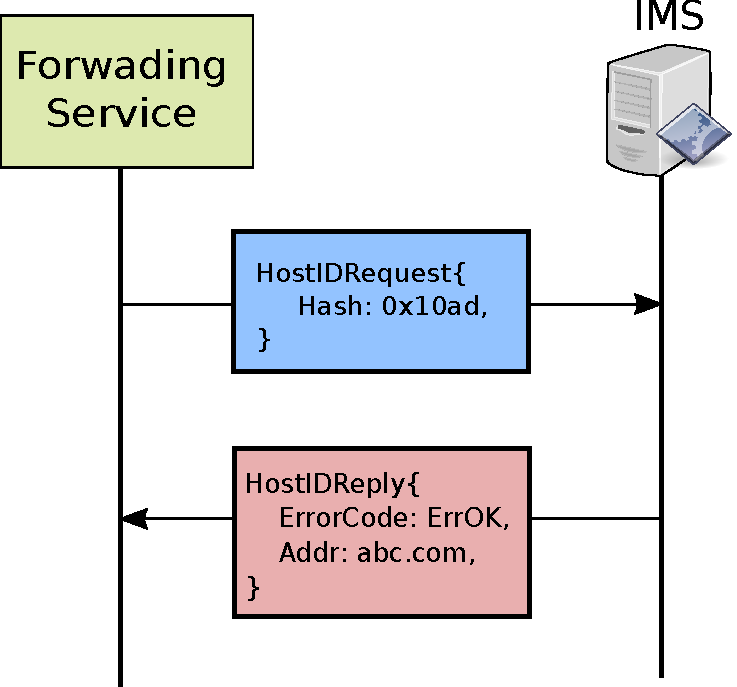
\includegraphics[scale=0.6]{Figures/siphash.pdf}
\decoRule
\caption[Host Identity Service]{Forwarding Service request IP address for a host identity from Identity Management Service (IMS)}
\label{fig:ims_request}
\end{figure}

\section{Implementation}
All the API access to APNA Management Service are modeled using Cap’n Proto specification.